%%% pruebas

\noindent Para este proyecto, se decidi\'o centrar las pruebas en dos tipos en espec\'ifico, pruebas de carga y pruebas de aceptaci\'on. Esto  debido a una limitante de tiempo, se eligieron entonces estas cargas ya que es vital garantizar que el sistema pudiera manejar m'ultiples solicitudes simult'aneamente sin comprometer su desempe\~no. Al igual que es de suma prioridad  asegurar que el sistema cumpliera con los requisitos funcionales y no funcionales definidos inicialmente, y que estos satisfacieran las expectativas del usuario final. 

\section{Pruebas de carga}
\noindent Haciendo uso del framework de pruebas Locust, que se enfoca en las pruebas de carga sobre aplicaciones web, se prob\'o simular quince usuarios simult\'aneos enviando m\'ultiples solicitudes de dietas suficientes en nutrientes (CoNA) con diferentes edades, esto para probar el desempe\~no del sistema en un escenario "realista" en el cual se cuenta con distintos usuarios de distintas edades solicitando dietas a la vez.

\begin{figure}[H]
    \centering
    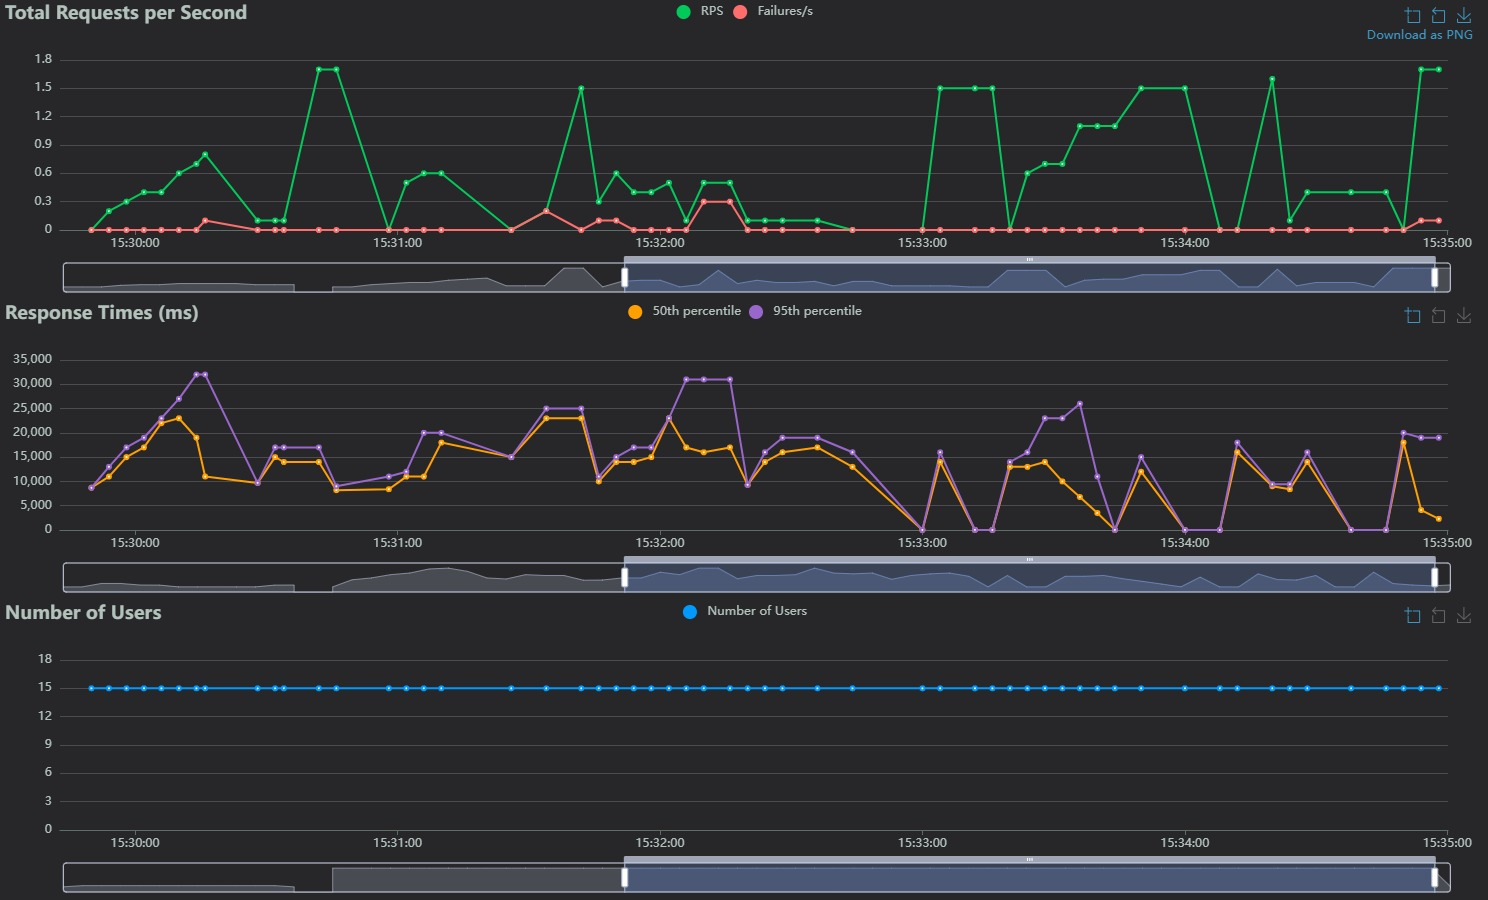
\includegraphics[height=8cm]{img/validacion/Carga.png}
    \caption{Prueba de carga}
    \label{fig:carga}
\end{figure}

En los resultados de la prueba, que se dej\'o corriendo durante cinco minutos, se puede observar que con un n\'umero de usuarios constantes la aplicaci\'on tiene tiempos de respuesta bastante elevados durante la mayor parte de la prueba, esto puede deberse a que ya que los c\'alculos no est\'an siendo realizados en el mismo servidor, sino en el servidor Plumber que se encuentra trabajando directamente con el paquete Foodprice, se est\'e generando un retraso en la comunicaci\'on del servidor de FastAPI y el de Plumber, ocasionando as\'i estos picos de respuesta tan elevados.
\\
\\
\section{Pruebas de aceptaci\'on}
\noindent Se realizaron pruebas con usuarios, con la colaboraci\'on de 7 conocidos y 8 personas desconocidas a trav\'es de diferentes d\'ias en los que se tuvo la oportunidad de que probaran la aplicaci\'on web de este proyecto; se les explic\'o de que va el proyecto, y lo b\'asico de su funcionamiento, pero se les incit\'o a que intentaran usar el sistema solo gui\'andose con las instrucciones de la aplicaci\'on, y despu\'es de utilizarla corriendo en mi computador personal, se les pidi\'o que llenaran una encuesta para conocer su opini\'on frente al sistema.
\\
\\
Estas pruebas se hicieron a trav\'es de una encuesta de google, en la que todos sus datos eran an\'onimos, para que tuvieran libertad de dar  su opinio\'on sincera.
\\
A continuaci\'on se plasman los resultados de dicha prueba:

\begin{figure}[H]
    \centering
    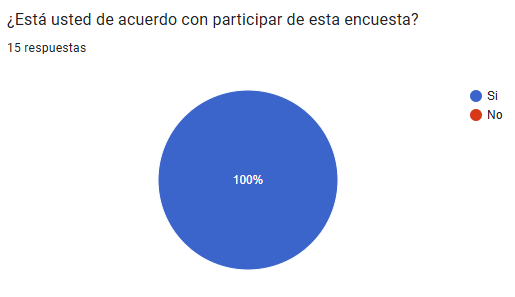
\includegraphics[height=8cm]{img/validacion/aceptacion.png}
    \caption{Prueba de aceptaci\'on 1}
    \label{fig:aceptacion1}
\end{figure}

\begin{figure}[H]
    \centering
    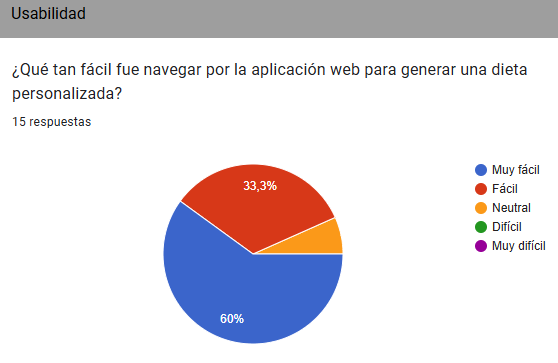
\includegraphics[height=8cm]{img/validacion/aceptacion2.png}
    \caption{Prueba de aceptaci\'on 2}
    \label{fig:aceptacion2}
\end{figure}

\begin{figure}[H]
    \centering
    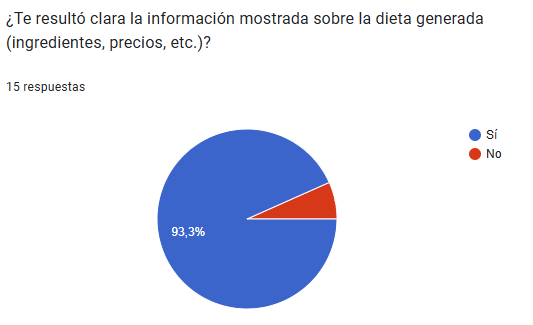
\includegraphics[height=8cm]{img/validacion/aceptacion3.png}
    \caption{Prueba de aceptaci\'on 3}
    \label{fig:aceptacion3}
\end{figure}

\begin{figure}[H]
    \centering
    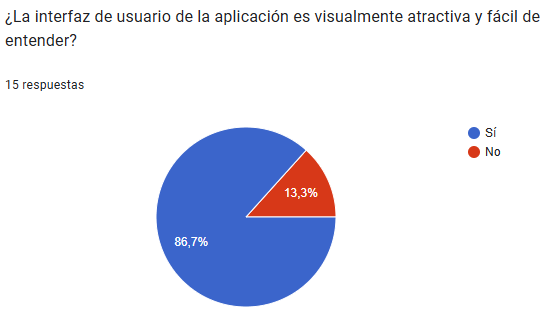
\includegraphics[height=8cm]{img/validacion/aceptacion4.png}
    \caption{Prueba de aceptaci\'on 4}
    \label{fig:aceptacion4}
\end{figure}

\begin{figure}[H]
    \centering
    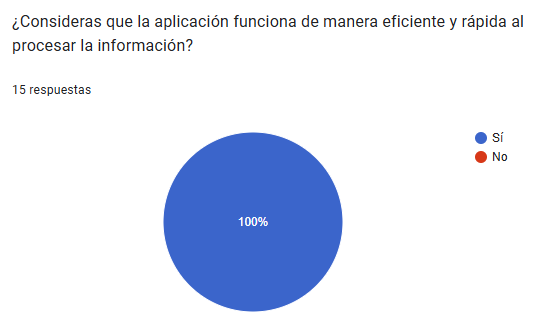
\includegraphics[height=8cm]{img/validacion/aceptacion5.png}
    \caption{Prueba de aceptaci\'on 5}
    \label{fig:aceptacion5}
\end{figure}

\begin{figure}[H]
    \centering
    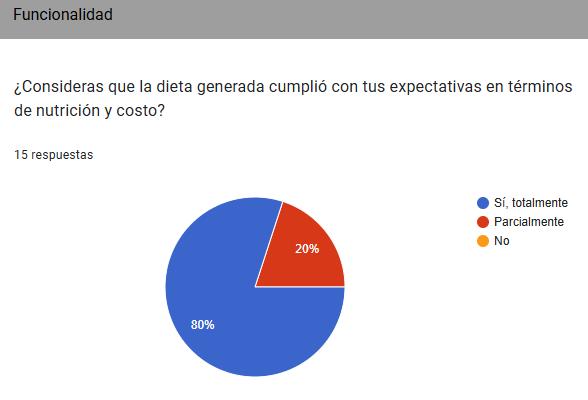
\includegraphics[height=8cm]{img/validacion/aceptacion6.png}
    \caption{Prueba de aceptaci\'on 6}
    \label{fig:aceptacion6}
\end{figure}

\begin{figure}[H]
    \centering
    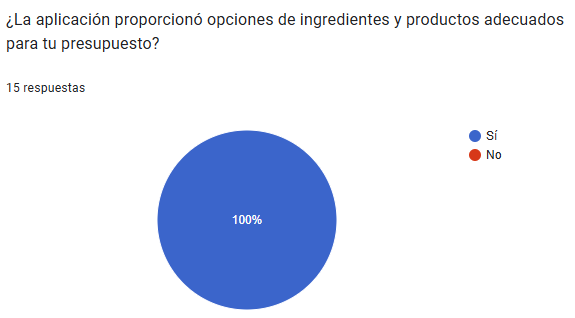
\includegraphics[height=8cm]{img/validacion/aceptacion7.png}
    \caption{Prueba de aceptaci\'on 7}
    \label{fig:aceptacion7}
\end{figure}

\begin{figure}[H]
    \centering
    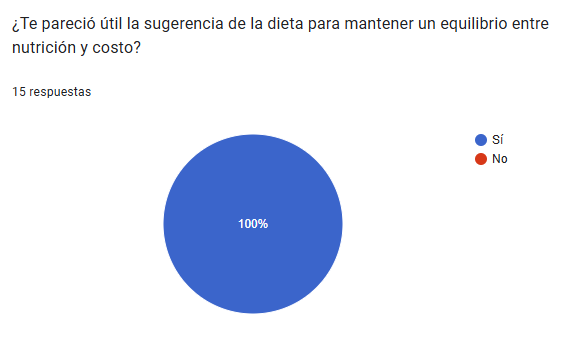
\includegraphics[height=8cm]{img/validacion/aceptacion8.png}
    \caption{Prueba de aceptaci\'on 8}
    \label{fig:aceptacion8}
\end{figure}

\begin{figure}[H]
    \centering
    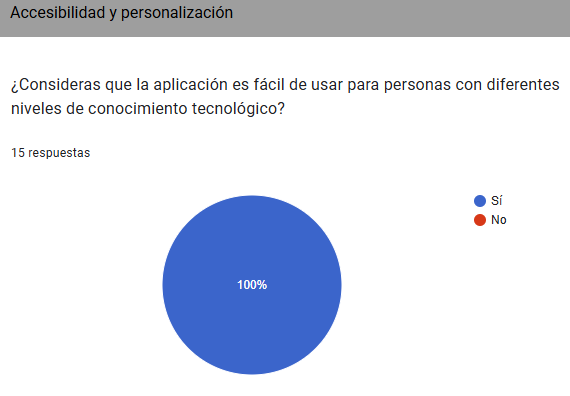
\includegraphics[height=8cm]{img/validacion/aceptacion9.png}
    \caption{Prueba de aceptaci\'on 9}
    \label{fig:aceptacion9}
\end{figure}

\begin{figure}[H]
    \centering
    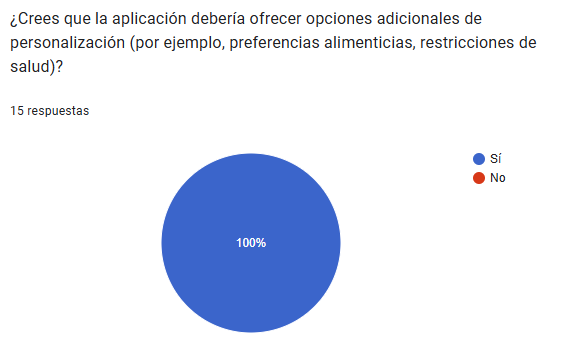
\includegraphics[height=8cm]{img/validacion/aceptacion10.png}
    \caption{Prueba de aceptaci\'on 10}
    \label{fig:aceptacion10}
\end{figure}

\begin{figure}[H]
    \centering
    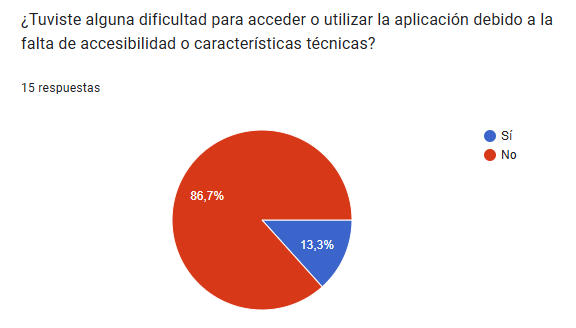
\includegraphics[height=8cm]{img/validacion/aceptacion11.png}
    \caption{Prueba de aceptaci\'on 11}
    \label{fig:aceptacion11}
\end{figure}

\begin{figure}[H]
    \centering
    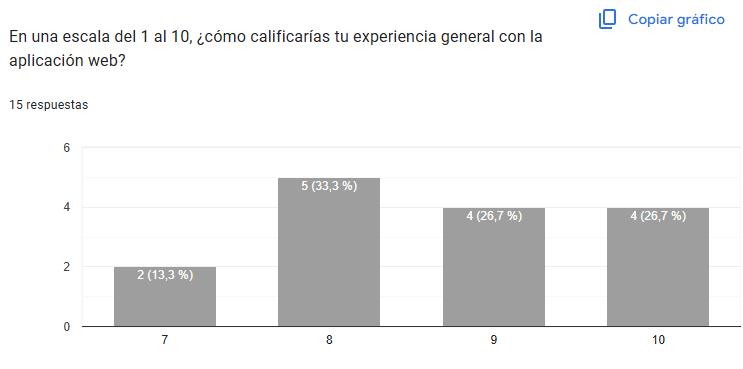
\includegraphics[height=8cm]{img/validacion/aceptacion12.png}
    \caption{Prueba de aceptaci\'on 12}
    \label{fig:aceptacion12}
\end{figure}

\begin{figure}[H]
    \centering
    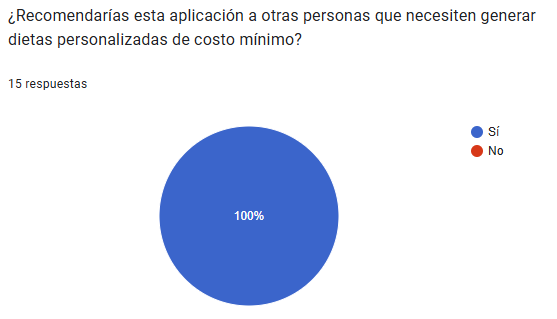
\includegraphics[height=8cm]{img/validacion/aceptacion13.png}
    \caption{Prueba de aceptaci\'on 13}
    \label{fig:aceptacion13}
\end{figure}

\begin{figure}[H]
    \centering
    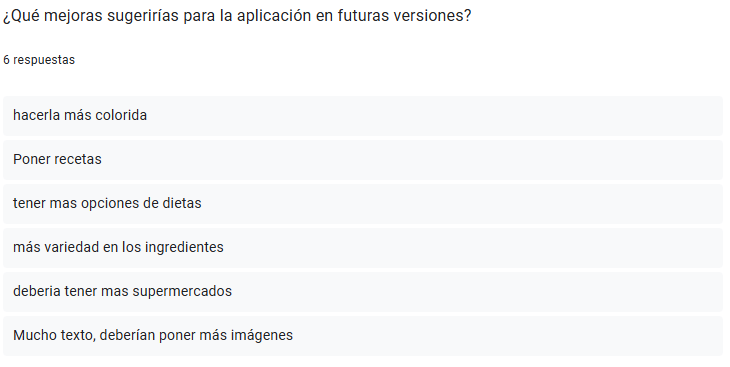
\includegraphics[height=8cm]{img/validacion/aceptacion14.png}
    \caption{Prueba de aceptaci\'on 14}
    \label{fig:aceptacion14}
\end{figure}

Con la informaci\'on recolectada a trav\'es de estas pruebas, se puede observar que el sistema tiene un nivel de aceptaci\'on bastante alto,  teniendo altos porcentajes de respuestas positivas frente a preguntas como la facilidad de navegaci\'on, la calificac\'on que le dan, entre otras.
\\
\\
Y las sugerencias son relacionadas no se centran en general en se\~nalar algo negativo que tenga el sistema, sino formas en las que les gustar\'ia a esos usuarios que el sistema incluyera m\'as cosas.
\\
\\
A futuro, ser\'ia ideal poder realizar pruebas de este estilo con una poblaci\'on que represente realmente la poblaci\'on que se quiere impactar con este proyecto; para as\'i medir realmente cual es el impacto en la vida de las personas.